\documentclass{article}

\usepackage[colorlinks=true]{hyperref}
\usepackage[utf8]{inputenc}
\usepackage[T1]{fontenc}
\usepackage[french]{babel}
\usepackage{graphicx}
\usepackage{float}
\usepackage{amsmath}
\usepackage{amssymb}
\usepackage{caption}
\usepackage{mathrsfs}
\usepackage{color}
\usepackage{fancyhdr}
\usepackage{pdfpages}
\usepackage{layout}
\usepackage{multicol}
\usepackage{setspace}
\usepackage[table]{xcolor}
\usepackage[top=1.5cm,bottom=1.5cm,left=0.45cm,right=0.45cm]{geometry}
\usepackage{amsthm}



%%%%%%%%%%%%%%%% Lengths %%%%%%%%%%%%%%%%
\setlength{\textwidth}{19cm}
\setlength{\evensidemargin}{-0,5cm}
\setlength{\oddsidemargin}{-0,5cm}

%%%%%%%%%%%%%%%% Variables %%%%%%%%%%%%%%%%
\def\projet{6}
\def\titre{Résolution approchée d'équations différentielles / Modélisation de systèmes dynamiques }
\def\groupe{2}
\def\equipe{8640}
\def\responsible{Benjamin UPTON}
\def\secretary{Anas TALBI}
\def\others{Aurélien MOINEL / Quentin LAMOUR / \\ \hspace{25.00mm} Ibrahim LMOURID}

\makeatletter
\newcommand\authorsection[2]{%
 \@ifstar\section\section*[#1]{#1 \hfill {\normalsize#2}}
}
\makeatother

\begin{document}

%%%%%%%%%%%%%%%% Header %%%%%%%%%%%%%%%%
\noindent\begin{minipage}{0.98\textwidth}
  \vskip 0mm
  \noindent
  { \begin{tabular}{p{7.5cm}}
      {\bfseries \sffamily
        Projet \projet} \\ 
      {\itshape \titre}
    \end{tabular}}
  \hfill 
  \fbox{\begin{tabular}{l}
      {~\hfill \bfseries \sffamily Groupe \groupe\ - Equipe \equipe
        \hfill~} \\[2mm] 
      Manager : \responsible \\
      Secrétaire : \secretary \\
      Programmeurs : \others
    \end{tabular}}
  \vskip 4mm ~

  ~~~\parbox{0.95\textwidth}{\small \textit{\textbf{Résumé}~: } \sffamily \\ Le but de ce projet est de s'intéresser aux méthodes de résolution d'équations différentielles ordinaires. Dans une première partie, nous présentons les méthodes de résolution à un pas afin de les utiliser sur des équations différentielles ordinaires en dimension finie. Ensuite, nous montrons deux applications de ces méthodes, à savoir le modèle de biologie des populations dit de Lokta-Volterra, et le pendule à $N$ maillons.
  }
  
\end{minipage}

%%%%%%%%%%%%%%%% Main part %%%%%%%%%%%%%%%%
\pagestyle{fancy}
\lhead{Algorithme Numérique}
\rhead{\thepage}
\lfoot{}
\cfoot{}
\rfoot{}
\vskip 3mm ~

\section{Méthodes numériques de résolution d'équations différentielles}
Dans cette partie, nous montrons les différentes méthodes de résolution numériques des équations différentielles afin d'en approximer les solutions.\\

\subsection{Algorithmes de résolution}

\textbf{Algorithme meth\_n\_step($y_0$, $t_0$, $N$, $f$, $step\_method$)}\\
Considérons l'intervalle $[t_0, t_f]$ représentant l'intervalle de temps durant lequel nous approximons la solution. Le but de cet algorithme consiste en la résolution de l'équation différentielle par calculs successifs des points $y_n$ au moment $t_n$. Pour ce faire, nous avons implémenté 4 méthodes de résolution différentes (Euler, Point milieu, Heun et Runge-Kutta d'ordre 4). Ces fonctions se présentent sous la forme \texttt{step\_<used\_method>($y_n$, $t_n$, $h$, $f$)}, avec $h$ le pas, et $f$ la fonction solution de $f(y,t) = y'(t)$. Le calcul de l'ensemble des points $y_0,...y_f$ correspondant à $N$ divisions de l'intervalle de départ, peuvent être calculés.\\

\textbf{Algorithme meth\_epsilon($y_0$, $t_0$, $N$, $f$, $step\_method$)}\\
Cet algorithme a pour but d'approximer une solution de l'équation différentielle avec une précision $\varepsilon$. Pour cela, calculons une première solution par le biais de l'algorithme précédent. Ensuite, nous nous approchons de la précision $\varepsilon$ grâce à une \textbf{boucle}. Cette boucle double $N$, et double la précision du pas $h$ à chaque itération. Ces nouvelles valeurs sont ensuite utilisées avec l'algorithme précédent pour calculer la nouvelle norme. Cette boucle est répétée tant que la précision $\varepsilon$ et le nombre maximum d'itérations ne sont pas atteints.

Cette méthode a pour avantage de rectifier la courbe de la pente à chaque itération, s'approchant de fait toujours plus de la solution exacte. Toutefois, toutes les méthodes ne se valent pas, par conséquent le nombre de points nécessaires pour approximer une solution avec une précision $\varepsilon$ fluctue.

\subsection{Tests des implémentations}
Afin de tester nos implémentations, nous avons tracer les solutions pour les deux équations différentielles \ref{eq:dim1} et \ref{eq:dim2} suivantes.

\begin{equation}
    \left\{
    \begin{array}{ll}
        y(0) &= 1 \\
        y'(t) &= \frac{y(t)}{1 + t^2}
    \end{array}
\right.
\label{eq:dim1}
\end{equation}

\begin{equation}
    \left\{
    \begin{array}{ll}
        y(0) &= \begin{bmatrix}
                    0 \\
                    1
                \end{bmatrix} \\
        y'(t) &= \begin{bmatrix}
                    -y_2(t) \\
                    y_1(t)
                \end{bmatrix} \\
    \end{array}
\right.
\label{eq:dim2}
\end{equation}

\begin{minipage}[c]{.46\linewidth}
    \centering
    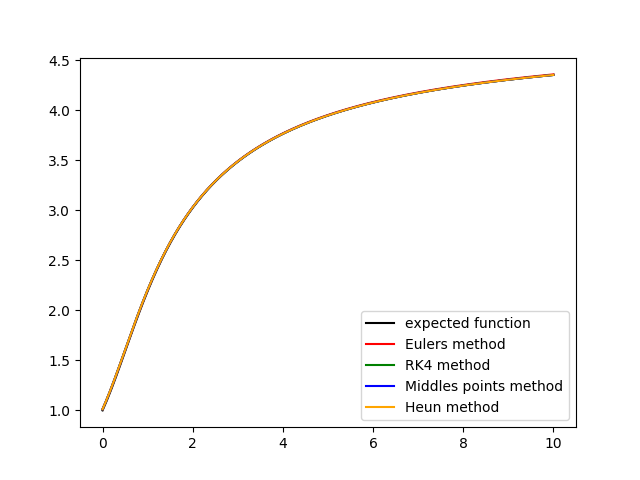
\includegraphics[scale=0.5]{images/dim1.png}
    \captionsetup{type=figure}\caption{Courbes solution de l'équation différentielle \ref{eq:dim1} pour $\varepsilon = 10^{-2}$ (solution exacte : $\exp\arctan(x)$)}
    \label{fig:dim1}
\end{minipage}
\hfill%
\begin{minipage}[c]{.46\linewidth}
    \centering
    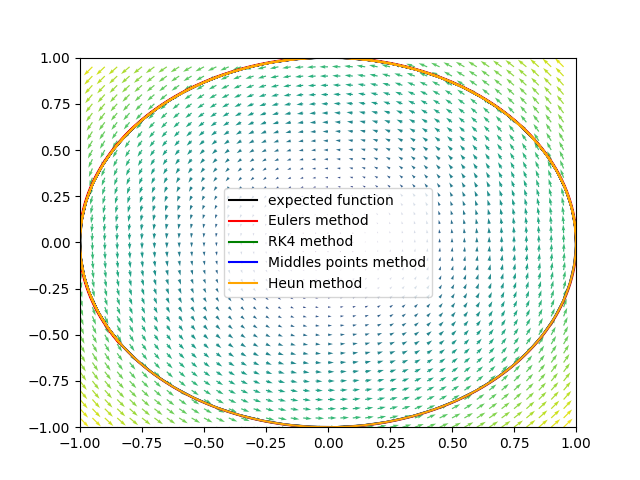
\includegraphics[scale=0.5]{images/dim2.png}
    \captionsetup{type=figure}\caption{Champs de tangentes et courbes solution de l'équation différentielle \ref{eq:dim2} pour $\varepsilon = 10^{-2}$
    (solution exacte : $[cos(x), sin(x)]$)}
    \label{fig:dim2}
\end{minipage}
\vspace{4.00mm}

On remarque nettement sur les deux figures \ref{eq:dim1}et \ref{eq:dim2} précédentes que toutes les méthodes convergent précisément vers la solution souhaitée dès lors que le $\varepsilon$ choisi est suffisamment précis.
De plus, on aperçoit sur la figure \ref{fig:dim2} que le champs de tangentes est suivi par l'approximation de nos solutions. Par conséquent, les méthodes semble correctement implémentées.

Néanmoins, nous avons rencontré des erreurs concernant les dimensions associées aux fonctions des équations différentielles. En effet, le code associé à l'algorithme \textbf{meth\_n\_step($y_0$, $t_0$, $N$, $f$, $step\_method$)} devait être implémenté de telle sorte à accepter ces différentes dimensions. De plus, comme nous l'avons évoqué précédemment pour l'algorithme \textbf{meth\_epsilon($y_0$, $t_0$, $N$, $f$, $step\_method$)} il était nécessaire d'ajouter une condition d'arrêt concernant le nombre d'itérations effectuées. En effet, son absence pouvait entraîner des boucles infinies dans le cas d'une non convergence.

\section{Système proie-prédateur de Lotka-Volterra}

L'objectif de cette partie est d'étudier l'évolution d'une population constituée par une ou plusieurs espèces.
\subsection{Modèles de Malthus et Verhulst}

\textbf{Malthus}\\

Considérons la fonction $N(t)$ qui décrit les variations d'une population au cours du temps. Dans le modèle de Malthus, cette fonction suit l'équation différentielle suivante :
\begin{align}
    \frac{dN(t)}{dt} &= bN(t) - dN(t) = \gamma N(t)
\end{align}
Ainsi, les taux de fertilité et de mortalité sont  considérés constants et proportionnels à la taille de la population $N(t)$. La Figure \ref{fig:Malthus} montre les variations de la fonction $N(t)$. \\% 

\textbf{Verhulst}\\

Ce modèle nous montre que le nombre d'individus de la population augmente exponentiellement lorsque le taux de naissances est plus élevé que le taux de mortalité. S'ils sont identiques, la population reste constante. Sinon, elle décroît jusqu'à son extinction. 


Dans ce modèle l'évolution de la population suit l'équation différentielle suivante :
\begin{align}
    \frac{dN(t)}{dt} &= \gamma N(t) (1 - \frac{N(t)}{K}) 
\end{align}
Le modèle de Verhulst est plus réaliste que le modèle de Malthus car il rajoute un coefficient qui limite la croissance de la population. \\

On remarque dans la Figure \ref{fig:Verhulst} que la population finit toujours par converger vers une valeur critique $K$.

\begin{minipage}[c]{.46\linewidth}
    \centering
    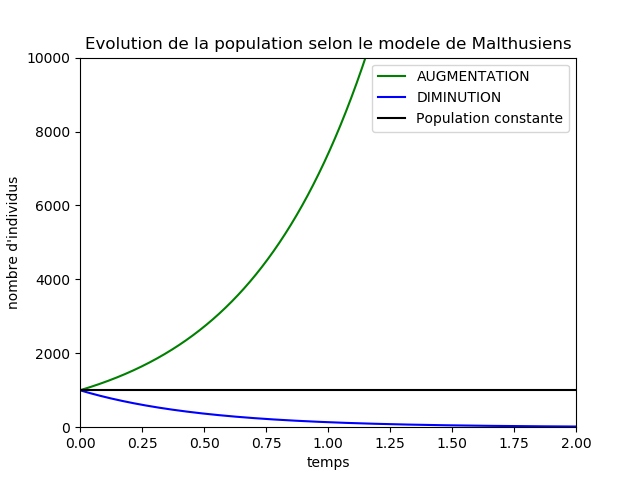
\includegraphics[scale=0.5]{images/Malthus.png}
    \captionsetup{type=figure}\caption{Évolution d'une population selon le modèle de Malthus}
    \label{fig:Malthus}
\end{minipage}
\hfill
\begin{minipage}[c]{.46\linewidth}
    \centering
    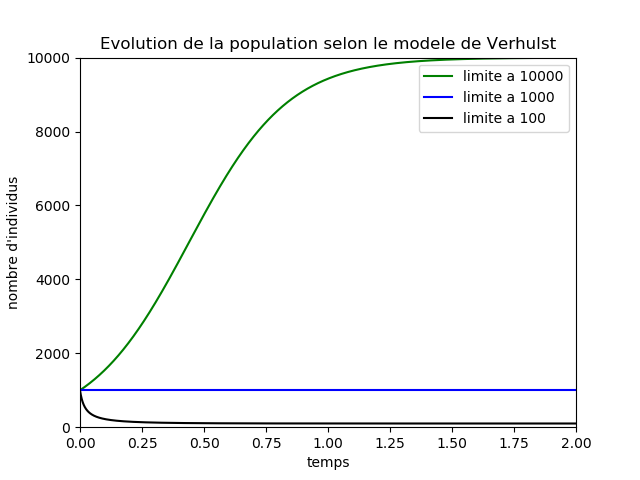
\includegraphics[scale=0.5]{images/Verhulst.png}
    \captionsetup{type=figure}\caption{Évolution d'une population selon le modèle de Verhulst}
    \label{fig:Verhulst}
\end{minipage}
\vspace{4.00mm}

\subsection{Modèle de Lotka-Volterra}
Les deux premiers modèles étudient l'évolution de la population sans prendre en compte les interactions entre les différentes espèces. Le modèle de Lotka-Volterra, modélise les interactions entre une population de proies, notée $N(t)$, et une population de prédateurs, notée $P(t)$, selon les deux équations différentielles suivantes :

\begin{align}
    \frac{dN(t)}{dt} &=  N(t) (a - bP(t)) \\
    \frac{dP(t)}{dt} &=  P(t) (cN(t) - d)
\end{align}

Ainsi, les proies se reproduisent indépendamment des prédateurs. Cependant, leur taux de mortalité est directement relié au nombre de prédateurs. De même, le taux de reproduction des prédateurs dépend des proies rencontrées, mais leur taux de mortalité est indépendant des proies. \\
\begin{minipage}[c]{.46\linewidth}
    \centering
    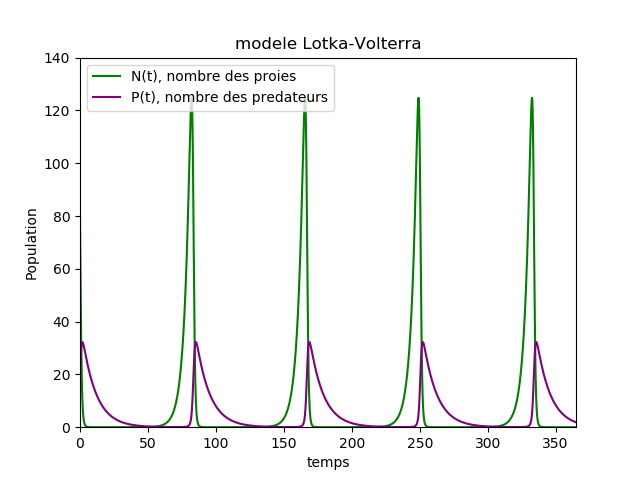
\includegraphics[width=\linewidth]{images/Lotka_Volterra.png}
    \captionsetup{type=figure}\caption{Évolution d'une population selon le modèle de Lotka\_Volterra}
    \label{fig:Lotka_Volterra}
\end{minipage}
\begin{minipage}[c]{.46\linewidth}
    \centering
    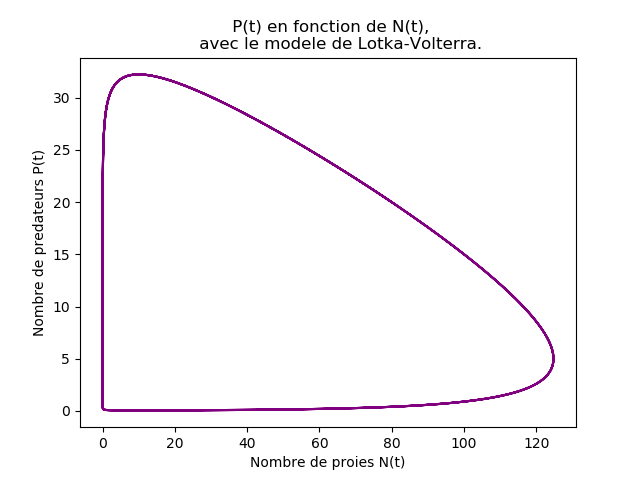
\includegraphics[width=\linewidth]{images/Lotka_Volterra_Pt_Nt.png}
    \captionsetup{type=figure}\caption{Évolution du nombre de prédateurs en fonction du nombre de proies.}
    \label{fig:Nt_Pt}
\end{minipage}
\hfill
\vspace{4.00mm}



D'après la Figure \ref{fig:Lotka_Volterra}, l'évolution des deux espèces est périodique et dépendante. En effet, le nombre de prédateurs augmente rapidement lorsqu'ils sont peu nombreux par rapport au nombre de proies. Par conséquent, le nombre de proies diminue entraînant par la suite une diminution du nombre de prédateurs. Enfin, le nombre de proies ré-augmente du fait qu'il y ait moins de prédateurs, et ainsi de suite.  

La Figure \ref{fig:Nt_Pt} représente le cycle de proie-prédateurs avec 80 proies et 20 prédateurs initialement. Cela correspond au nombre de prédateur en fonction du nombre de proies au cours du temps. On peut constater que l'évolution des 2 populations est cyclique donc infinie : c'est le modèle de cohabitation des espèces, les 2 espèces cohabitent ensemble sans ne jamais s'éteindre. Nous pouvons noter également que la Figure \ref{fig:Nt_Pt} représente $P(t)$ en fonction de $N(t)$ lorsque ces deux fonctions sont des solutions non constantes de l'équation différentielle. D'ailleurs, il existe deux solutions constantes :

\begin{align}
    N(t) &= 0, P(t)=0  \\
    N(t) &= \frac{d}{c}, P(t)=\frac{a}{b}
\end{align}

\begin{minipage}[c]{.46\linewidth}
    \centering
    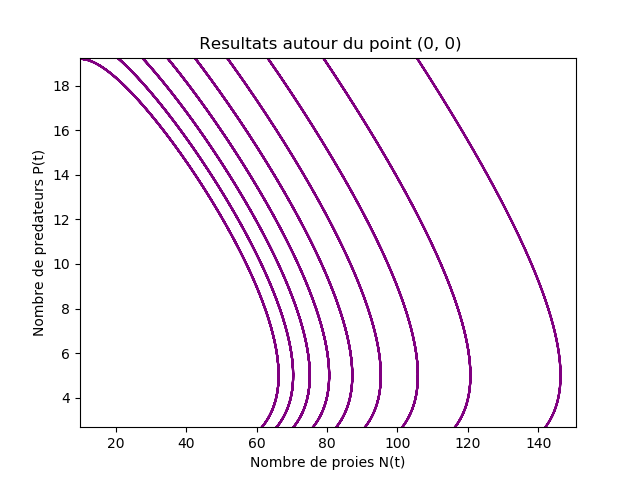
\includegraphics[width=\linewidth]{images/zoom.png}
    \captionsetup{type=figure}\caption{Comportement local au point (0, 0)}
    \label{fig:zoom}
\end{minipage}
\hfill
\begin{minipage}[c]{.46\linewidth}
    \centering
    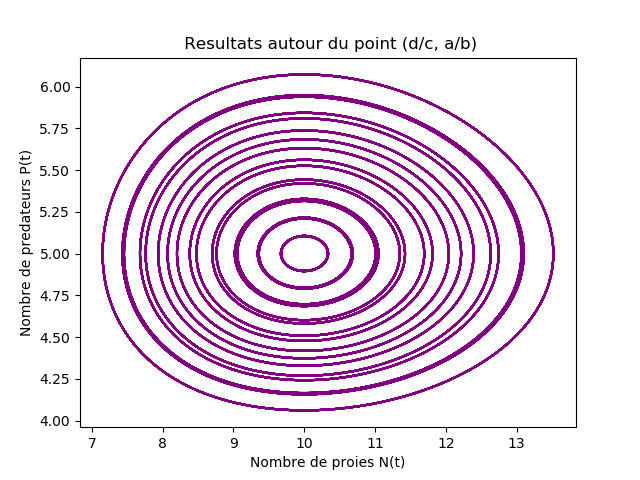
\includegraphics[width=\linewidth]{images/singulier.png}
    \captionsetup{type=figure}\caption{Comportement local au point (d/c, a/b)}
    \label{fig:singulier}
\end{minipage}
\vspace{4.00mm}

Les deux Figures \ref{fig:zoom} et \ref{fig:singulier} montrent que les solutions autour d'un point non singulier, ou bien autour du point $(0,0)$, sont sous la forme d'arcs qui entourent le point. Cependant, les solutions autour du point $(d/c, a/b)$ sont sous la forme de cercles qui entourent le point.


\section{Pendule à N maillons}

Cette section aborde le cas du pendule à $N$ maillons, et plus spécifiquement le cas du pendule simple et du pendule double.

\subsection{Simple pendule}

Un simple pendule correspond à une masse $m$ (ponctuelle) attachée à l'extrémité d'un fil de longueur $l$ sans masse et inextensible qui oscille sous l'effet de la gravité.

Considérons un pendule de masse $m$, de longueur $l$, et d'angle $\theta$ par rapport à la verticale. L'équation différentielle \ref{eq:simple_pendulum} ci-dessous est obtenu par l'application du \textbf{Principe Fondamental de la Dynamique} (PFD) sur $m$.
\begin{align}
    \frac{d\varepsilon}{dt} &= 0 \\
    \varepsilon &= \varepsilon_k + \varepsilon_p \\
    \varepsilon_k &= \frac{1}{2}mv^2 \text{avec $v = l\dot{\theta}$} \\
    &\text{soit $\varepsilon_k = \frac{1}{2}ml^2\dot{\theta}^2$} \\
    &\text{et $\theta = \frac{\pi}{2}, \varepsilon_p = -mgl \cos{\theta}$} \\
    \varepsilon &= \frac{1}{2}ml^2\dot{\theta}^2 - mgl\cos{\theta} \\
    \frac{d\varepsilon}{dt} &= ml^2\dot{\theta}\ddot{\theta} + mgl \sin{\theta\dot{\theta}} \\
    &\text{d'où $\boxed{\ddot{\theta} = \frac{g}{l}\sin{\theta}}$}
    \label{eq:simple_pendulum}
\end{align}

En considérant de faibles oscillations, ainsi que le développement de $\sin$ au voisinage de zéro (premier ordre), on a alors l'équation différentielle $\ddot{\theta} = -\frac{g}{l}\sin{\theta}$. La résolution de celle-ci se fait par l'utilisation des méthodes évoquées précédemment, et plus spécifiquement la méthode de \textbf{Runge-Kutta d'ordre 4} dans notre cas.

On considère le vecteur 
\vspace{4.00mm}

\begin{equation}
    X(t) = \begin{pmatrix} \theta(t) \\ \dot{\theta}(t) \end{pmatrix}
\end{equation}
, d'où 
\begin{equation}
    X'(t) = \begin{pmatrix} \ddot{\theta}(t) \\ \frac{g}{l}\sin{\theta(t)} \end{pmatrix} = f(t, X(t))
    \label{eq:dif_simple_pendulum}
\end{equation}


Comme expliqué précédemment, nous avons utilisé la méthode de \textbf{Runge-Kutta d'ordre 4} pour obtenir la variation de l'angle $\theta$ en fonction du temps (Figure \ref{fig:var_theta}). Ensuite, nous avons réalisé le tracé de la variation de la fréquence en fonction de l'angle initial $\theta_0$ (Figure \ref{fig:var_freq}), tout en utilisant la méthode \textbf{Runge-Kutta d'ordre 4}. En outre, on remarque que pour un petit angle $\theta$, la fréquence s'approche de $\frac{\sqrt{g}}{2*\pi*\sqrt{l}}$

\begin{minipage}[c]{.46\linewidth}
    \centering
    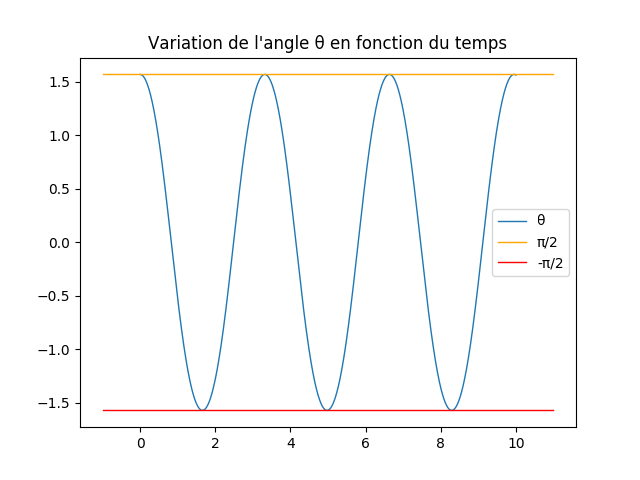
\includegraphics[width=\linewidth]{images/var_theta.png}
    \captionsetup{type=figure}\caption{Variation de l'angle $\theta$ en fonction du temps (Résolution de l'équation différentielle \ref{eq:dif_simple_pendulum} pour $m = 1kg$, $l = 1m$, $g = 9.81m/s^2$) et $\theta_0 = \frac{\pi}{2}$.}
    \label{fig:var_theta}
\end{minipage}
\hfill%
\begin{minipage}[c]{.46\linewidth}
    \centering
    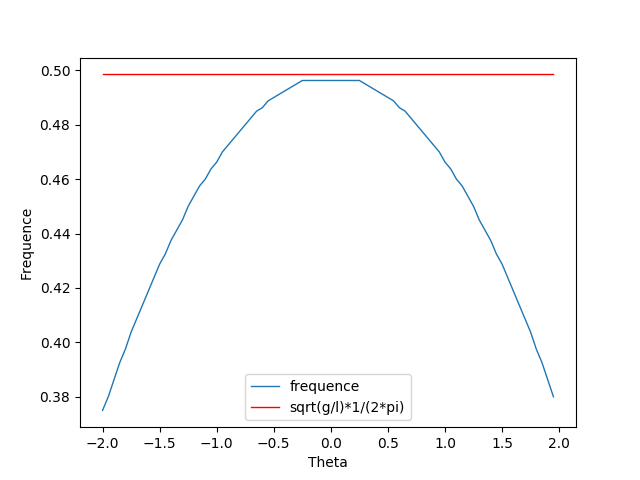
\includegraphics[width=\linewidth]{images/var_freq.png}
    \captionsetup{type=figure}\caption{Variation de la fréquence d'oscillation en fonction de l'angle initial $\theta_0$ (pour $m = 1kg$, $l = 1m$, $g = 9.81m/s^2$).}
    \label{fig:var_freq}
\end{minipage}


\subsection{Double pendule}
Le double pendule consiste en l'ajout d'un second pendule simple de longueur $l_2$ et de masse $m_2$ au niveau de la masse du premier pendule.

Ainsi, on utilise la même méthode que précédemment pour résoudre le système. On considère le vecteur : 

\vspace{4.00mm}
\begin{equation}
    X(t) = \begin{pmatrix} \theta_1(t) \\ \dot{\theta_1}(t) \\ \theta_2(t) \\ \dot{\theta_2}(t) \end{pmatrix}
\end{equation}
, d'où 
\begin{equation}
    X'(t) = \begin{pmatrix} \dot{\theta_1}(t) \\ \frac{-g(2m_1 + m_2)\sin{\theta_1(t)}-m_2g\sin(\theta_1(t)-2\theta_2(t))-2\sin(\theta_1(t) - \theta_2(t))m_2(\omega^{2}_2L_2+\omega^{2}_1L_1\cos(\theta_1(t) - \theta_2(t)))}{L_1(2m_1+m_2-m_2\cos(2\theta_1(t) - 2 \theta_2(t)))} \\ \dot{\theta_2}(t) \\ \frac{2\sin(\theta_1(t) - \theta_2(t))(\omega^{2}_1L_1(m_1+m_2)+g(m_1 + m_2)\cos{\theta_1(t)} + \omega^{2}_2L_2m_2\cos(\theta_1(t) - \theta_2(t)))}{L_2(2m_1+m_2-m_2\cos(2\theta_1(t) - 2 \theta_2(t)))} \end{pmatrix}
\end{equation}

Ainsi, nous pouvons simuler la trajectoire de l'extrémité du pendule à deux maillons en fonction du temps tel que montré sur la figure \ref{fig:trace_double_pendulum}. On remarque également sur cette figure, que la légère variation de l'angle $\theta_1$ ou $\theta_2$ provoque de grand changement sur la trajectoire. Ainsi, cela démontre la dépendance du système aux conditions initiales. Ce comportement est normal, car inhérent aux systèmes chaotiques dont fait parti le double pendule (du fait des deux équations différentielles liées).

\begin{minipage}[c]{.46\linewidth}
    \centering
    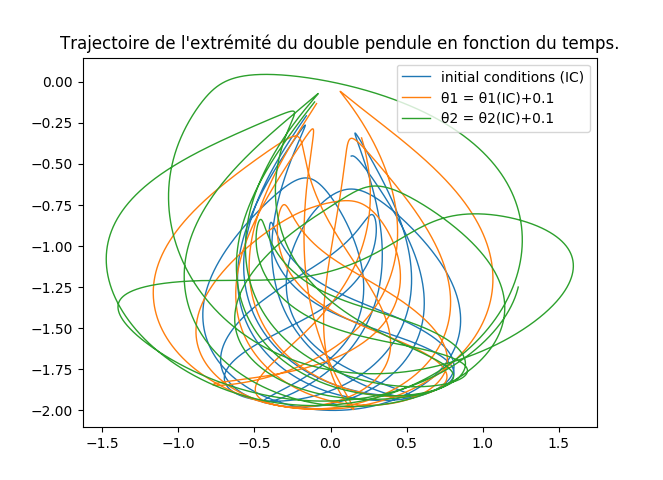
\includegraphics[width=\linewidth]{images/trace_pendule.png}
    \captionsetup{type=figure}\caption{Conditions initiales : $m_1 = m_2 = 1kg$, $l_1 = l_2 = 1 m$, $g = 9.81m/s^2$}
    \label{fig:trace_double_pendulum}
\end{minipage}
\hfill%
\begin{minipage}[c]{.46\linewidth}
    \centering
    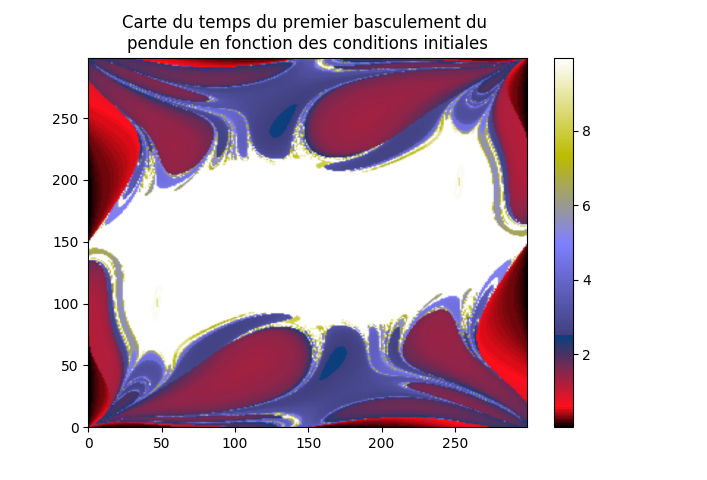
\includegraphics[width=\linewidth]{images/map_time.png}
    \captionsetup{type=figure}\caption{Conditions initiales : $m_1 = m_2 = 1kg$, $l_1 = l_2 = 1 m$, $g = 9.81m/s^2$) sur une période de $10$ secondes}
    \label{fig:map_time}
\end{minipage}
\vspace{4.00mm}

Enfin, un autre moyen permettant de mettre en avant les propriétés du système consistait en la création d'une carte du temps du premier basculement du pendule en fonction du temps (Figure \ref{fig:map_time}). Par temps de basculement, nous entendons le temps nécessaire pour que l'angle $\theta_1$ du premier pendule ou l'angle $\theta_2$ du second pendule dépasse $\pi$. De part les variations de couleurs, on remarque rapidement qu'il devient très compliqué de prévoir les mouvements du double pendule. En effet, pour un changement minime de $\theta$, le temps de basculement peut se produire bien plus tardivement, voir jamais.


\section{Conclusion}
Pour conclure, ce projet a mis en avant l'efficacité des méthodes de résolution d'équations différentielles ordinaires pour certaines applications. Nous avons également mesuré l'importance de la généricité du code en raison des dimensions différentes associées aux fonctions de ces équations. Ensuite, nous avons abordé deux applications différentes, mais avoir le temps de toutes les traitées aurait pu donner un plus large aperçu de la puissance de résolution liée aux méthodes implémentées. Enfin, nous avons été en mesure de constater la difficulté de prédire certains comportements relatifs aux systèmes chaotiques, dus à leurs dépendances aux conditions initiales.

\end{document}
%%% Local Variables:
%%% mode: latex
%%% TeX-master: t
%%% End:

